% Asset ID: AS2StatisticalDistributionsTikZ-004
% Source: Chapter 6 Statistical Distributions transcript, cumulative probability section
% Related lesson section: Core Theory 8.6, Worked Examples 10-13, Exam Technique Notes
% Purpose: Cumulative binomial probability conversion map.

\documentclass[tikz,border=8pt]{standalone}
\usepackage{amsmath}
\usetikzlibrary{positioning, arrows.meta}

\begin{document}
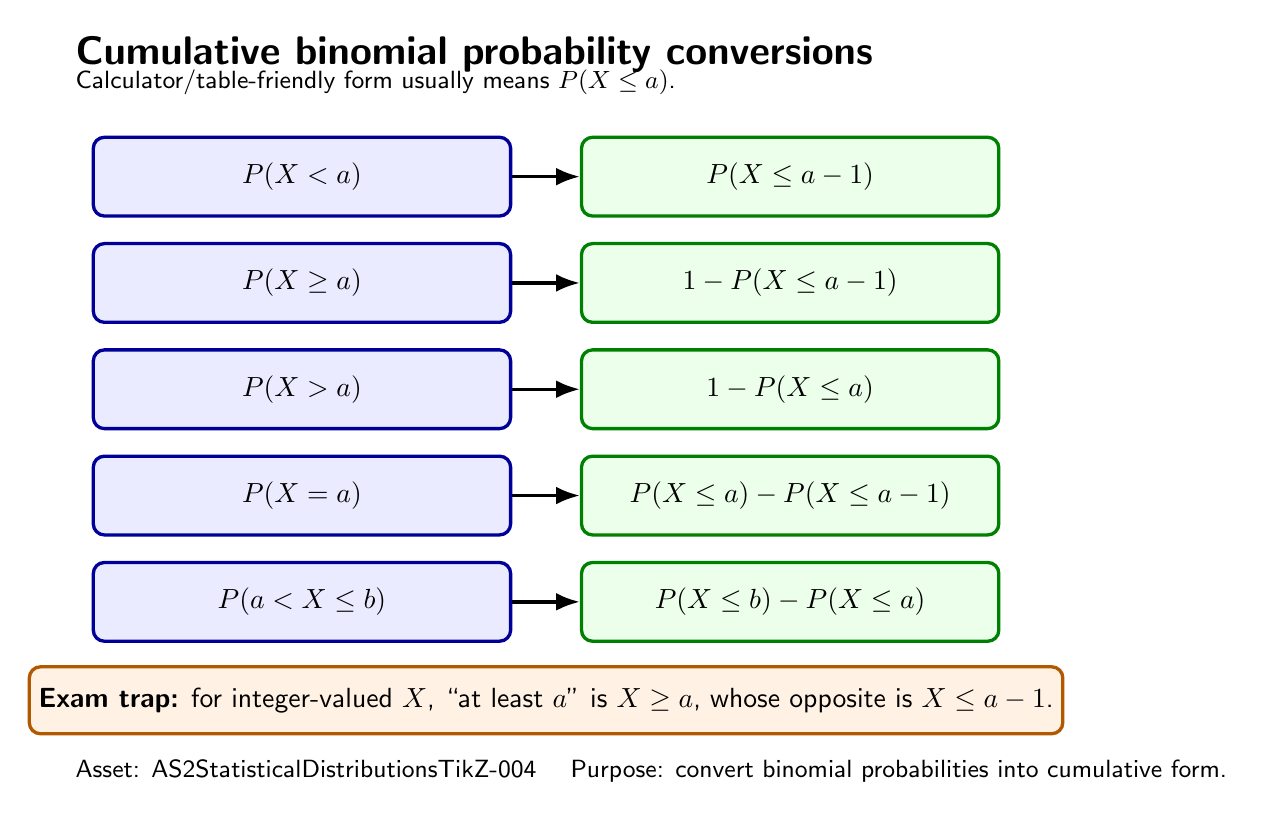
\begin{tikzpicture}[conv/.style={draw=black,very thick,rounded corners,fill=white,align=center,font=\sffamily,minimum width=5.3cm,minimum height=1.0cm},left/.style={conv,fill=blue!8,draw=blue!60!black},right/.style={conv,fill=green!8,draw=green!50!black},warn/.style={draw=orange!70!black,fill=orange!10,very thick,rounded corners,align=center,font=\sffamily,minimum width=11.5cm,minimum height=0.85cm},arrow/.style={very thick, -{Latex[length=3mm]}},title/.style={font=\sffamily\bfseries\Large},subtitle/.style={font=\sffamily\small}]
\node[anchor=west, title] at (-6.1,4.35) {Cumulative binomial probability conversions};
\node[anchor=west, subtitle] at (-6.1,4.0) {Calculator/table-friendly form usually means $P(X\le a)$.};
\node[left] (a1) at (-3.1,2.8) {$\displaystyle P(X<a)$};\node[right] (b1) at (3.1,2.8) {$\displaystyle P(X\le a-1)$};\draw[arrow] (a1) -- (b1);
\node[left] (a2) at (-3.1,1.45) {$\displaystyle P(X\ge a)$};\node[right] (b2) at (3.1,1.45) {$\displaystyle 1-P(X\le a-1)$};\draw[arrow] (a2) -- (b2);
\node[left] (a3) at (-3.1,0.1) {$\displaystyle P(X>a)$};\node[right] (b3) at (3.1,0.1) {$\displaystyle 1-P(X\le a)$};\draw[arrow] (a3) -- (b3);
\node[left] (a4) at (-3.1,-1.25) {$\displaystyle P(X=a)$};\node[right] (b4) at (3.1,-1.25) {$\displaystyle P(X\le a)-P(X\le a-1)$};\draw[arrow] (a4) -- (b4);
\node[left] (a5) at (-3.1,-2.6) {$\displaystyle P(a<X\le b)$};\node[right] (b5) at (3.1,-2.6) {$\displaystyle P(X\le b)-P(X\le a)$};\draw[arrow] (a5) -- (b5);
\node[warn] at (0,-3.85) {\textbf{Exam trap:} for integer-valued $X$, ``at least $a$'' is $X\ge a$, whose opposite is $X\le a-1$.};
\node[anchor=west, subtitle] at (-6.1,-4.75) {Asset: AS2StatisticalDistributionsTikZ-004 \quad Purpose: convert binomial probabilities into cumulative form.};
\end{tikzpicture}
\end{document}
